\chapter{Эксперимент 2: Сравнение эффективности ссылочных и векторных структур}

\section{Цель эксперимента}
Оценить влияние зависимости команд по данным на эффективность вычислений.

\section{Описание проблемы}
Обработка зависимых данных происходит в тех случаях, когда результат работы одной команды используется в качестве адреса операнда другой. При программировании на языках высокого уровня такими операндами являются указатели, активно используемые при обработке ссылочных структур данных: списков, деревьев, графов. Обработка данных структур процессорами с длинными конвейерами команд приводит к заметному увеличению времени работы алгоритмов: адрес загружаемого операнда становится известным только после обработки предыдущей команды. В противоположность этому, обработка векторных структур, таких как массивы, позволяет эффективно использовать аппаратные возможности ЭВМ. 

\section{Суть эксперимента}
Для сравнения эффективности векторных и списковых структур в эксперименте применяется профилировка кода двух алгоритмов поиска минимального значения. Первый алгоритм использует для хранения данных список, в то время как во втором применяется массив. Очевидно, что время работы алгоритма поиска минимального значения в списке зависит от его фрагментации, т.е. от среднего расстояния между элементами списка. 

\section{Условия эксперимента}
\begin{enumerate}
    \item Единицы измерения по Ох - Килобайты;
    \item Единицы измерения по Оу - Такты;
    \item Количество элементов в списке: \textbf{1};
    \item Максимальная фрагментация списка: \textbf{256};
    \item Шаг изменения фрагментации: \textbf{4};
\end{enumerate}

\section{Результаты эксперимента}
\begin{figure}[ht!]
    \centering
    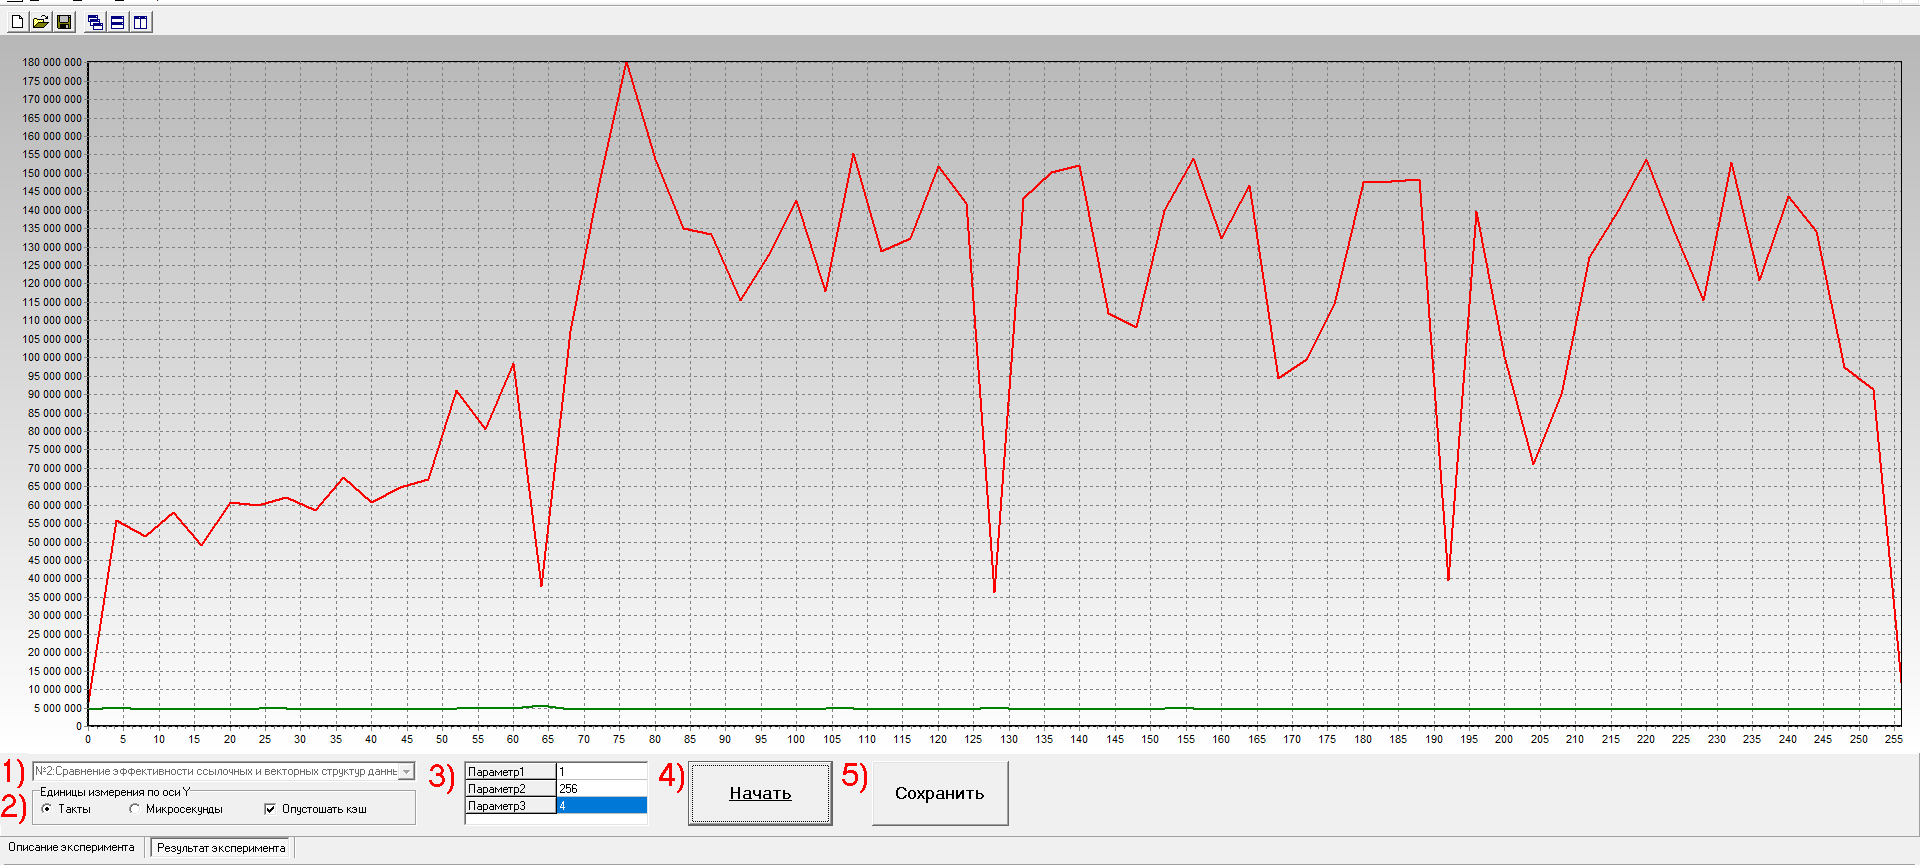
\includegraphics[width=170mm]{./img/2.png}
    \caption{Эксперимент 2: Сравнение эффективности ссылочных и векторных структур}
\end{figure}

\begin{figure}[ht!]
    \centering
    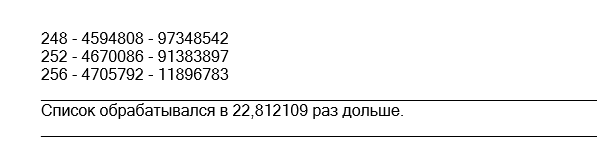
\includegraphics[width=100mm]{./img/02.png}
    \caption{Эксперимент 2: Результаты}
    \label{res_02}
\end{figure}

Как видно из рисунка \ref{res_02}: массив обрабатывается примерно в 20-30 раз быстрее списка.

\section{Вывод}
Из полученных результатов следует, что при выборе структуры данных нужно учитывать технологические факторы конкретной задачи. 
Если задача позволяет использовать массив, то им следует воспользоваться, если использование списка не принесет значительных выгод, особенно в плане времени.